\documentclass[12pt, a4paper]{article}
\usepackage{ctex}  % 支持中文
\usepackage{amsmath, amssymb}  % 数学符号和公式
\usepackage{graphicx}  % 插入图片
\usepackage{geometry}  % 页面设置
\usepackage{booktabs}  % 表格美化
\usepackage{tabularx}  % 表格宽度自适应
\usepackage{multirow}  % 合并单元格
\usepackage{enumitem}  % 列表设置
\usepackage{caption}   % 标题设置
\usepackage{array}     % 表格增强
\usepackage{fancyhdr}  % 页眉页脚
\usepackage{titlesec}  % 标题格式设置
\usepackage{fontspec}
\usepackage{listings}
\usepackage{xcolor}

\usepackage[
  backend=bibtex,
  style=gb7714-2015,   % 使用中国国标格式,适合中文论文
  sorting=none         % 按引用顺序排序
]{biblatex}

\addbibresource{references.bib} % 参考文献配置

% 页面设置
\geometry{left=2.5cm, right=2.5cm, top=2.5cm, bottom=2.5cm}

% 重定义section格式为居中
\titleformat{\section}{\centering\Large\bfseries}{\thesection}{1em}{}
\titleformat{\subsection}{\normalsize\bfseries}{\thesubsection}{1em}{}
\titleformat{\subsubsection}{\normalsize\bfseries}{\thesubsubsection}{1em}{}

% 表格表头格式
\renewcommand{\thetable}{\arabic{section}.\arabic{table}}

% 设置表格标题格式:左对齐,中文带"表"字,表题加粗
\captionsetup[table]{
  labelsep=space,
  labelformat=simple,
  textfont=bf,
  labelfont=bf,
  name=表
}

% 图片编号格式
\renewcommand{\thefigure}{\arabic{section}-\arabic{figure}}

% 设置图片标题格式
\captionsetup[figure]{
  labelsep=space,
  labelformat=simple,
  textfont=bf,     
  labelfont=bf, 
  position=bottom,  
  name=图
}

% 修改公式编号格式
\renewcommand{\theequation}{\thesection-\arabic{equation}}

% 参考文献格式
\makeatletter
\renewcommand\@biblabel[1]{[#1]}
\makeatother

% 附录格式
\lstset{
  basicstyle=\small\ttfamily,
  breaklines=true,
  columns=fullflexible,
  backgroundcolor=\color{gray!10},
  frame=single,
  rulecolor=\color{black!30},
  commentstyle=\color{green!50!black},
  keywordstyle=\color{blue},
  stringstyle=\color{red},
  numbers=left,
  numberstyle=\tiny\color{gray},
  numbersep=5pt
}


\begin{document}

% 标题部分
\begin{center}
\LARGE\textbf{中国股市FF三因子资产定价模型的实证检验}

\vspace{1cm}
\large 计金220 22011854 高菻铠
\end{center}

\noindent \textbf{摘要:} 本文基于2009-2017年中国A股市场七个行业指数及2004-2023的个股数据,对Fama-French三因子资产定价模型进行系统性实证检验,旨在探究该模型在中国市场的适用性及中国股市的独特定价特征。研究结果表明,从行业指数角度看,单资产时间序列检验与GRS联合检验均显示三因子模型能够较好地解释行业指数的超额收益,行业间风险暴露存在显著异质性,如银行业表现出低市场风险、负规模敏感性和正价值敏感性,而电气设备、化工等行业则呈现高市场风险、正规模敏感性和负价值敏感性。然而,在个股层面,序贯排序分析揭示出中国股市存在显著的反向规模效应和反向价值效应,即大市值股票收益率高于小市值股票,成长型股票表现优于价值型股票,这与经典Fama-French模型的结论相反。Fama-MacBeth横截面回归分析进一步证实了上述发现,对数流通市值系数显著为正,盈利价格比系数显著为负,表明市值和盈利价格比对股票收益率具有显著解释力。此外,CAPM中的Beta系数虽整体显著为正,但其显著性在近期有所减弱。研究结果表明,中国股市的资产定价机制具有独特性,传统基于美国市场的多因子模型在中国市场存在局限性,需发展本土化资产定价模型,同时为投资者提供了在中国市场配置大市值成长型股票的理论依据。

\section{文献综述}

金融资产定价理论是现代金融经济学的重要组成部分,其中资本资产定价模型(CAPM)作为资产定价理论的重要基石之一,受到了广泛的关注与深入的研究。Fama和French在1993年提出的三因子模型进一步拓展了CAPM模型,引入了规模因子(SMB)和账面市值比因子(HML),以更好地解释股票收益率的横截面差异。然而,随着资本市场的不断发展,该模型的适用性在不同市场中受到质疑,尤其是在新兴市场中。近年来,Fama和French在2015年提出的五因子模型进一步引入了盈利能力因子(RMW)和投资风格因子(CMA),以期更全面地解释股票收益率的差异。

在中国市场,\citet{zhang2014ff}对2001-2011年沪深两市的数据进行了实证检验,发现规模、账面市值比、市盈率倒数与股票收益率呈负相关,而贝塔系数和财务杠杆与收益率呈正相关。这一研究结果表明,传统的CAPM模型在中国市场中存在局限性,而三因子模型在中国市场中具有一定的适用性。然而,\citet{zhao2016fama}对2003-2014年中国A股市场的数据进行分析后发现,Fama-French五因子模型中的RMW和CMA因子在中国市场中并不显著,而三因子模型的解释能力更强。这表明在中国市场中,盈利能力因子和投资风格因子可能并不像在美国市场中那样重要。

进一步地,\citet{li2017fama}对1994-2015年中国A股市场的数据进行了分析,发现股权分置改革前后,五因子模型的适用性存在显著差异。股改前,市场风险占据主导地位,盈利能力、投资风格及动量因子“冗余”;股改后,这些因子的风险溢价显著,且存在经五因子模型调整后仍然显著的反转效应。这一研究表明,随着中国资本市场的制度变革,资产定价模型的适用性也会发生变化。

在国际比较方面,\citet{carpenter2021real}研究了中国股票市场的价格信息含量和资本配置效率,发现自2004年以来,中国股票价格对未来的利润预测能力与美国相当,且这种信息含量对私人企业的投资效率提升有显著作用。然而,对于国有企业,尤其是在2008年金融危机后的刺激政策期间,价格信息含量和投资效率均有所下降。这一研究结果表明,中国股票市场在信息传递和资本配置方面具有一定的价值,但不同所有制企业的表现存在差异。

此外,\citet{liu2019size}对中国股票市场的规模效应和价值效应进行了深入研究,发现中国市场的规模效应和价值效应显著,且使用收益-价格比(EP)构建的价值因子比账面市值比(BM)更能捕捉中国市场的价值效应。他们还发现,排除潜在的壳价值干扰后,规模和价值因子在中国市场的表现优于传统的Fama-French三因子模型。这一研究结果进一步证实了中国股票市场在资产定价方面的独特性。

综合上述研究可以发现,中国股票市场在资产定价方面具有其独特性,传统的CAPM模型和Fama-French三因子模型在中国市场的适用性受到一定限制。随着中国资本市场的不断发展和完善,资产定价模型需要考虑更多的市场特征和投资者行为因素。因此,深入研究中国股票市场的收益率分布特征和影响因素,对于理论探索和实践投资策略的制定都具有重要意义。

\section{数据与方法}

\subsection{数据描述}

本研究使用中国A股市场2009年至2017年的数据,从锐思数据库和Tushare数据库获取七个行业指数的周度数据以及中国股市的月度数据。选取的七个申万行业指数包括:银行(801780.SI)、化工(801030.SI)、钢铁(801040.SI)、有色金属(801050.SI)、建筑材料(801710.SI)、电气设备(801730.SI)和医药生物(801150.SI)。此外,我们还获取了三因子模型所需的月度因子数据。

对于横截面检验,我们收集了2004-2023年所有A股股票的月度收益率、流通市值数据、市盈率数据以及CAPM风险因子Beta数据。市场组合收益率使用沪深300指数(000300.SH)的周度和月度收益率作为代理,无风险利率则采用中国人民银行公布的相应期限国债收益率。

数据预处理包括异常值处理、缺失值填补和变量计算。特别地,我们计算了盈利价格比(市盈率的倒数)作为价值因子的衡量指标,并对流通市值取对数以减小其尺度影响。所有变量均进行了1\%和99\%分位数的缩尾处理,以减轻极端值对分析结果的影响。

\subsection{Fama-French三因子模型检验方法}

\subsubsection{单资产时间序列检验}

对每个行业指数,我们首先进行FF三因子模型的时间序列回归,模型设定如下:

\begin{equation}
R_{i,t} - R_{f,t} = \alpha_i + \beta_i(R_{m,t} - R_{f,t}) + s_i\text{SMB}_t + h_i\text{HML}_t + \varepsilon_{i,t}
\end{equation}

其中,$R_{i,t}$为行业$i$在时间$t$的收益率,$R_{f,t}$为无风险收益率,$R_{m,t}$为市场收益率,$\text{SMB}_t$和$\text{HML}_t$分别为规模因子和价值因子。$\alpha_i$、$\beta_i$、$s_i$和$h_i$为待估计参数,$\varepsilon_{i,t}$为随机扰动项。

计算三因子时,我们按照Fama-French(1993)的方法,先按市值将股票分为大小两组,再按账面市值比(使用市盈率倒数作为代理变量)将股票分为高、中、低三组,形成六个投资组合。SMB因子为小市值三个组合的平均收益率减去大市值三个组合的平均收益率;HML因子为高账面市值比两个组合的平均收益率减去低账面市值比两个组合的平均收益率。

对每个行业,我们估计上述模型并检验$\alpha_i$是否显著不为零。如果$\alpha_i$不显著,且模型的整体F检验显著,则认为该行业满足FF三因子模型。

\subsubsection{多资产联合检验}

为验证FF三因子模型对所有七个行业的解释能力,我们采用Gibbons-Ross-Shanken(GRS)检验方法进行多资产联合检验。GRS统计量计算如下:

\begin{equation}
\text{GRS} = \left(\frac{T-N-K}{N}\right) \left(1 + \hat{\mu}' \hat{\Omega}^{-1} \hat{\mu}\right)^{-1} \hat{\alpha}' \hat{\Sigma}^{-1} \hat{\alpha}
\end{equation}

其中,$T$为样本容量,$N$为资产数量,$K$为因子数量,$\hat{\mu}$为因子均值向量,$\hat{\Omega}$为因子协方差矩阵,$\hat{\alpha}$为截距项向量,$\hat{\Sigma}$为残差协方差矩阵。

GRS检验的原假设为所有行业的$\alpha_i$同时为零。在显著性水平为5\%下,如果无法拒绝原假设,则表明FF三因子模型能够很好地解释这些行业的超额收益率。

\subsection{序贯排序法检验}

本研究采用Fama-French(1992)中提出的序贯排序方法,研究市值和盈利价格比对股票收益率的联合影响。序贯排序法是资产定价研究中常用的非参数检验方法,能直观展示不同特征组合的收益率差异。

在实证过程中,我们对每个月的股票数据首先按照流通市值大小进行排序,将样本均分为5个投资组合,从最小市值组合到最大市值组合。随后,在每个市值分组内,再按照盈利价格比(市盈率的倒数)从高到低进行排序,进一步将每个市值组分为5个子组合,形成高盈利价格比(价值型)到低盈利价格比(成长型)的谱系。通过这种两维排序,我们构建了共计25个投资组合。

对于每个投资组合,我们计算其月平均收益率,并对研究期间(2004-2023年)的数据取时间序列平均值,最终形成5×5的排序结果表格。此表格的行代表不同市值分组,列代表不同盈利价格比分组,单元格数值则表示相应投资组合的平均月收益率。

通过分析结果表格中的收益率模式,特别是行方向和列方向的边际收益率差异,我们可以识别中国A股市场中市值效应和价值效应的存在性及其相互作用关系。例如,如果最小市值组合的平均收益率显著高于最大市值组合,则表明存在显著的小市值效应;同样,如果高盈利价格比组合的平均收益率显著高于低盈利价格比组合,则表明存在显著的价值效应。

\subsection{Fama-MacBeth回归检验}

本研究采用Fama-MacBeth(1973)两阶段回归方法检验市值、盈利价格比和CAPM Beta对股票收益率的解释能力。Fama-MacBeth回归首先考察每个月份的横截面关系,随后对时间序列上的系数进行统计推断,该方法能有效处理截面相关性问题,在资产定价实证研究中被广泛应用。

在方法的第一阶段,我们对每个月份$t$的横截面数据进行OLS回归。回归模型设定如下:

\begin{equation}
R_{i,t} = \gamma_{0,t} + \gamma_{1,t}\beta_{i} + \gamma_{2,t}\ln(\text{ME}_{i,t}) + \gamma_{3,t}\text{E/P}_{i,t} + \epsilon_{i,t}
\end{equation}
其中,$R_{i,t}$表示股票$i$在月份$t$的收益率,$\beta_i$代表股票$i$的CAPM Beta值,$\ln(\text{ME}_{i,t})$为对数流通市值,$\text{E/P}_{i,t}$为盈利价格比。通过回归,我们获得了每个月份的横截面系数估计值$\gamma_{k,t}$。

方法的第二阶段则着眼于对上述系数的时间序列进行统计分析。我们计算各系数在时间维度上的平均值:

\begin{equation}
\bar{\gamma}_k = \frac{1}{T}\sum_{t=1}^{T}\gamma_{k,t}
\end{equation}
随后,我们通过计算t统计量评估各系数的统计显著性:

\begin{equation}
t(\bar{\gamma}_k) = \frac{\bar{\gamma}_k}{\sigma(\gamma_{k,t})/\sqrt{T}}
\end{equation}

其中,$\bar{\gamma}_k$为第$k$个系数的时间序列平均值,$\sigma(\gamma_{k,t})$为其标准差,$T$为样本中包含的月份数量。

我们不仅对整个样本期间(2004-2023年)进行分析,还将其划分为两个子期间(2004-2013年和2014-2023年)进行比较,以检验各因素效应的稳健性和时变特性。

\subsection{模型评估与稳健性分析}

我们通过多种指标评估模型拟合效果。对时间序列回归,主要考察调整后的$R^2$和F统计量;对Fama-MacBeth回归,则关注各系数的时间序列平均显著性及其在不同子期间的稳定性。

为增强结果稳健性,我们对各变量进行了1\%和99\%分位数缩尾处理,并剔除了市盈率为负或极端的观测值。在计算Beta值时,我们采用了36个月的滚动窗口方法,对于数据不足的情况则使用全样本估计,同时对异常Beta值进行了修正处理。

所有分析均使用Python实现,回归分析采用statsmodels库,数据处理和可视化分别使用pandas、numpy和matplotlib等工具包。

\section{实证结果}

\subsection{FF三因子模型的单资产时间序列检验}

本研究基于2009至2017年的周度数据对七个行业指数进行了系统性分析,首先通过单资产时间序列回归方法,评估Fama-French三因子模型对各行业指数超额收益率的解释能力。表\ref{tab:ff_single_test}呈现了各行业的三因子模型估计结果。

\begin{table}[htbp]
\centering
\caption{各行业FF三因子模型回归结果}
\label{tab:ff_single_test}
\begin{tabular}{lccccc}
\toprule
行业 & $\alpha$ & $\beta_{MKT}$ & $\beta_{SMB}$ & $\beta_{HML}$ & $R^2$ \\
\midrule
银行 & -0.0010 & 0.8810*** & -0.2508*** & 0.2868*** & 0.674 \\
 & (-0.9180) & (27.8214) & (-4.1067) & (5.7946) & \\
化工 & -0.0021 & 1.0339*** & 0.9800*** & -0.4834*** & 0.694 \\
 & (-1.6336) & (26.3125) & (12.9317) & (-7.8723) & \\
钢铁 & -0.0020 & 1.0681*** & 0.6041*** & 0.0887 & 0.662 \\
 & (-1.6048) & (27.7815) & (8.1471) & (1.4766) & \\
有色金属 & -0.0014 & 1.1537*** & 0.8392*** & -0.3241*** & 0.695 \\
 & (-1.0516) & (28.4639) & (10.7356) & (-5.1158) & \\
建筑材料 & -0.0018 & 1.0779*** & 0.8362*** & -0.3708*** & 0.725 \\
 & (-1.4872) & (30.0962) & (12.1048) & (-6.6246) & \\
电气设备 & -0.0021 & 1.1287*** & 1.0310*** & -0.5391*** & 0.637 \\
 & (-1.3027) & (23.2700) & (11.0212) & (-7.1115) & \\
\bottomrule
\multicolumn{6}{l}{\scriptsize 注:括号内为t统计量;***、**、*分别表示在1\%、5\%和10\%的水平上显著。}
\end{tabular}
\end{table}

对单资产时间序列回归结果的分析表明,所有行业的截距项($\alpha$)均不显著异于零,支持了Fama-French三因子模型对这些行业收益率的良好解释能力。市场因子($\beta_{MKT}$)在所有行业均呈现显著的正系数,数值范围在0.88至1.15之间,表明这些行业对市场普遍呈现较强敏感性。值得注意的是,银行行业的市场$\beta$系数最低(0.88),反映了该行业相对较低的系统性风险特征;而有色金属行业的市场$\beta$系数最高(1.15),说明其对市场波动的高度敏感性。

规模因子($\beta_{SMB}$)在大多数行业显示出显著的正系数,银行业为明显例外,其SMB系数为显著负值(-0.25)。本差异揭示了银行板块与其他行业在规模特征上的本质区别:银行业主要由大市值股票构成,其收益率表现与小市值股票呈现负相关性;而其他行业,特别是电气设备(1.03)和化工(0.98)则呈现出与小市值股票更为相似的收益模式。

价值因子($\beta_{HML}$)则呈现出更为复杂的行业异质性。银行业对HML因子表现出显著正向敏感性(0.29),表明其具有典型的价值型特征;而电气设备、化工和建筑材料行业对HML因子的敏感性则显著为负,分别为-0.54、-0.48和-0.37,体现出这些行业的成长型特征。钢铁行业是唯一一个HML系数不显著的行业,表明其收益率与价值因子相对独立。

\begin{figure}[htbp]
\centering
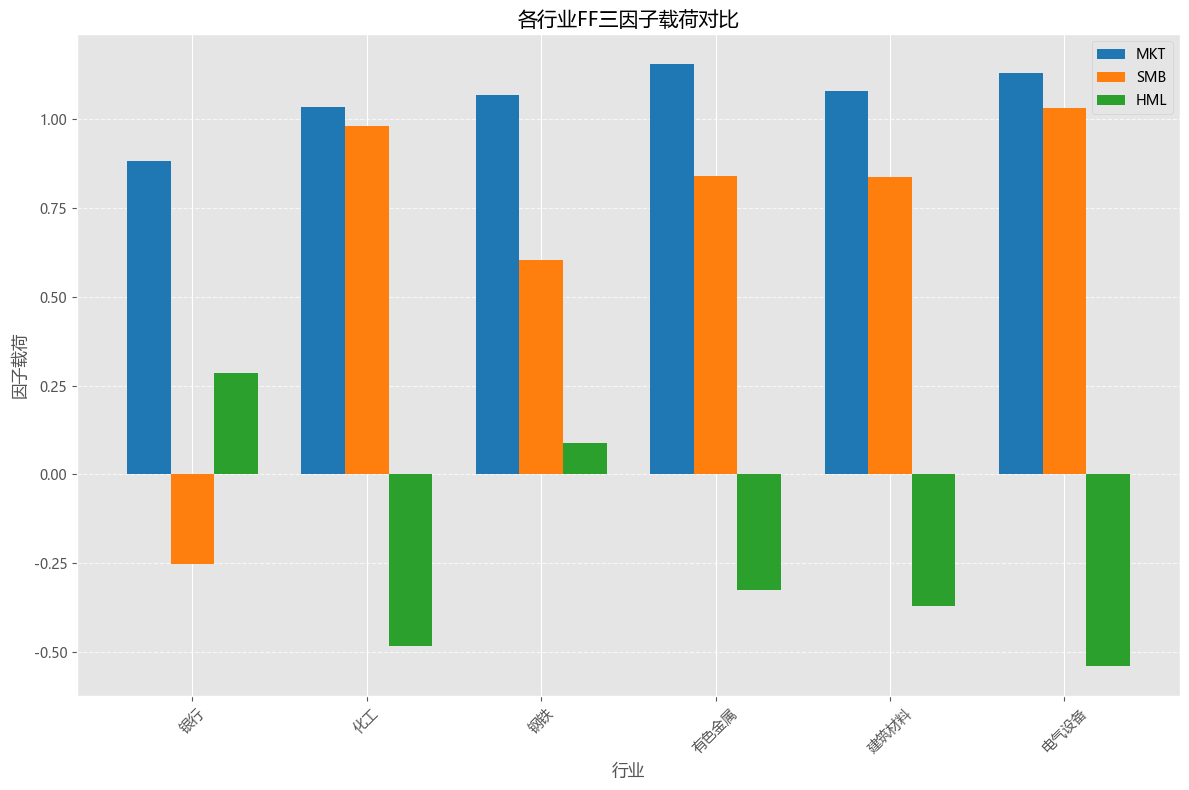
\includegraphics[width=0.8\textwidth]{./img/各行业FF三因子载荷对比.png}
\caption{各行业FF三因子载荷对比}
\label{fig:factor_loadings}
\end{figure}

图\ref{fig:factor_loadings}直观展示了各行业对三个因子的敏感性差异,清晰呈现了行业间存在的风险暴露异质性。从市场风险角度看,所有行业均呈现出较高的系统性风险暴露;从规模效应看,除银行外,其他行业均表现出对小市值溢价的正向暴露;从价值维度看,行业间差异最为显著,形成了以银行为代表的价值型板块与以电气设备为代表的成长型板块的鲜明对比。

模型的整体解释力度方面,各行业的调整R方均在0.63至0.72之间,其中建筑材料行业的拟合优度最高(0.725),而电气设备行业最低(0.637)。这表明FF三因子模型能够解释这些行业超过60\%的收益率波动,体现了该模型在中国市场中具有相当的解释力。图\ref{fig:r_square}直观展示了各行业拟合优度的对比,所有行业的R方均在0.63以上,进一步证实了该模型在中国A股市场中解释行业超额收益时间序列变化的适用性。

\begin{figure}[htbp]
\centering
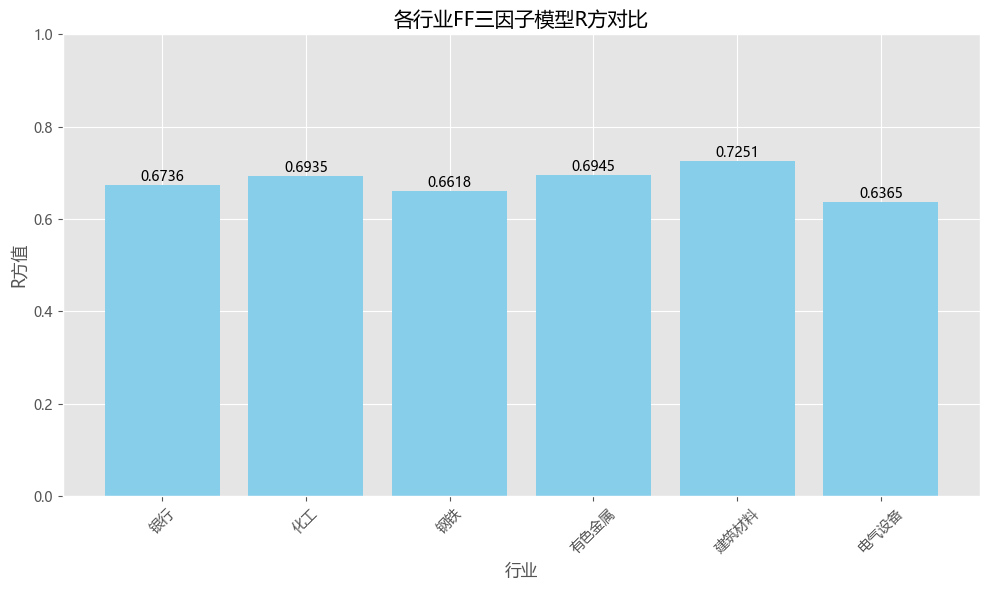
\includegraphics[width=0.8\textwidth]{./img/各行业R方对比.png}
\caption{各行业FF三因子模型的拟合优度对比}
\label{fig:r_square}
\end{figure}

\subsection{FF三因子模型的多资产联合检验}

为进一步验证FF三因子模型的有效性,本研究在单资产检验的基础上,采用Gibbons-Ross-Shanken(GRS)检验进行多资产联合检验。表\ref{tab:grs_test}展示了GRS联合检验的详细结果。

\begin{table}[htbp]
\centering
\caption{FF三因子模型的GRS联合检验结果}
\label{tab:grs_test}
\begin{tabular}{lcc}
\toprule
检验项目 & 统计量 & 评价 \\
\midrule
GRS统计量 & 1.3429 & \multirow{3}{*}{不能拒绝所有$\alpha$=0的假设} \\
p值 & 0.2367 & \\
5\%临界值 & 2.1252 & \\
\midrule
资产数量(N) & 6 & \multirow{3}{*}{样本充足} \\
观测期数(T) & 459 & \\
因子数量(K) & 3 & \\
\midrule
所有$\alpha$的平均绝对值 & 0.0017 & 经济显著性低 \\
所有$\alpha$的平方和 & 0.0000126 & 整体偏离程度小 \\
\bottomrule
\end{tabular}
\end{table}

GRS检验结果显示,统计量为1.34,对应p值为0.24,显著低于5\%显著性水平下的临界值2.13,因此无法拒绝"所有行业$\alpha$值同时为零"的原假设。所有行业$\alpha$值的平均绝对值仅为0.0017,表明各行业收益率对三因子模型的偏离程度在经济上也不显著。这一结果进一步支持了FF三因子模型对中国股市行业收益差异的解释能力,表明三因子系统性风险已能充分解释样本期间内各行业的超额收益率。

进一步分析各行业在联合检验框架下的表现,我们发现尽管个别行业(如化工和钢铁)的单资产检验中$\alpha$的t值接近显著水平,但在考虑因子收益的时变特性和残差的横截面相关性后,整体检验无法拒绝模型的有效性。这种现象反映了单资产检验和多资产联合检验在统计功效上的差异,也突显了多资产联合框架在评估资产定价模型时的重要性。

多资产检验结果与单资产检验形成互补,共同表明Fama-French三因子模型在解释中国行业指数收益方面具有显著能力。市场、规模和价值三个系统性风险因素能够捕捉大部分行业收益的横截面和时间序列变化,上述发现为构建以行业为基础的投资组合和风险管理策略提供了理论依据。

值得一提的是,虽然三因子模型在解释行业指数层面表现良好,但正如后续分析将展示的,当考察个股层面的定价机制时,中国股市可能存在与经典理论预期不一致的现象,这反映了中国股市微观结构与成熟市场的差异性。

\subsection{市值与盈利价格比的序贯排序分析}

本研究采用序贯排序法分析了市值因素与盈利价格比(市盈率的倒数)对股票收益率的联合影响,通过构建二维排序投资组合,揭示中国A股市场在2004至2023年间的规模效应与价值效应。表\ref{tab:sequential_sorting}展示了按市值和盈利价格比序贯排序后得到的25个投资组合的平均月收益率。

\begin{table}[htbp]
\centering
\caption{按市值和盈利价格比的序贯排序结果(月平均收益率)}
\label{tab:sequential_sorting}
\begin{tabular}{cccccc|c}
\toprule
\multirow{2}{*}{市值分组} & \multicolumn{5}{c|}{盈利价格比分组(从高到低)} & \multirow{2}{*}{市值组平均} \\
 & 1(价值型) & 2 & 3 & 4 & 5(成长型) & \\
\midrule
1(小) & -0.0060 & 0.0018 & 0.0047 & 0.0070 & 0.0045 & 0.0024 \\
2 & -0.0016 & 0.0065 & 0.0080 & 0.0097 & 0.0154 & 0.0076 \\
3 & -0.0016 & 0.0069 & 0.0116 & 0.0134 & 0.0198 & 0.0100 \\
4 & 0.0041 & 0.0073 & 0.0124 & 0.0164 & 0.0206 & 0.0122 \\
5(大) & 0.0069 & 0.0068 & 0.0168 & 0.0248 & 0.0213 & 0.0153 \\
\hline
盈利价格比组平均 & 0.0004 & 0.0059 & 0.0107 & 0.0143 & 0.0163 & 0.0095 \\
\bottomrule
\end{tabular}
\end{table}

序贯排序结果揭示了中国股市存在显著的反向规模效应和反向价值效应。从市值维度看,平均月收益率随着市值增加而单调递增,从小市值组合的0.24\%逐步上升至大市值组合的1.53\%。最大市值组合与最小市值组合之间1.29\%的月度收益率差异(年化约15.48\%)明确表明中国股市存在显著的反向规模效应,即大市值股票系统性优于小市值股票,这与经典Fama-French模型中小市值股票获得风险溢价的发现形成鲜明对比。

\begin{figure}[htbp]
\centering
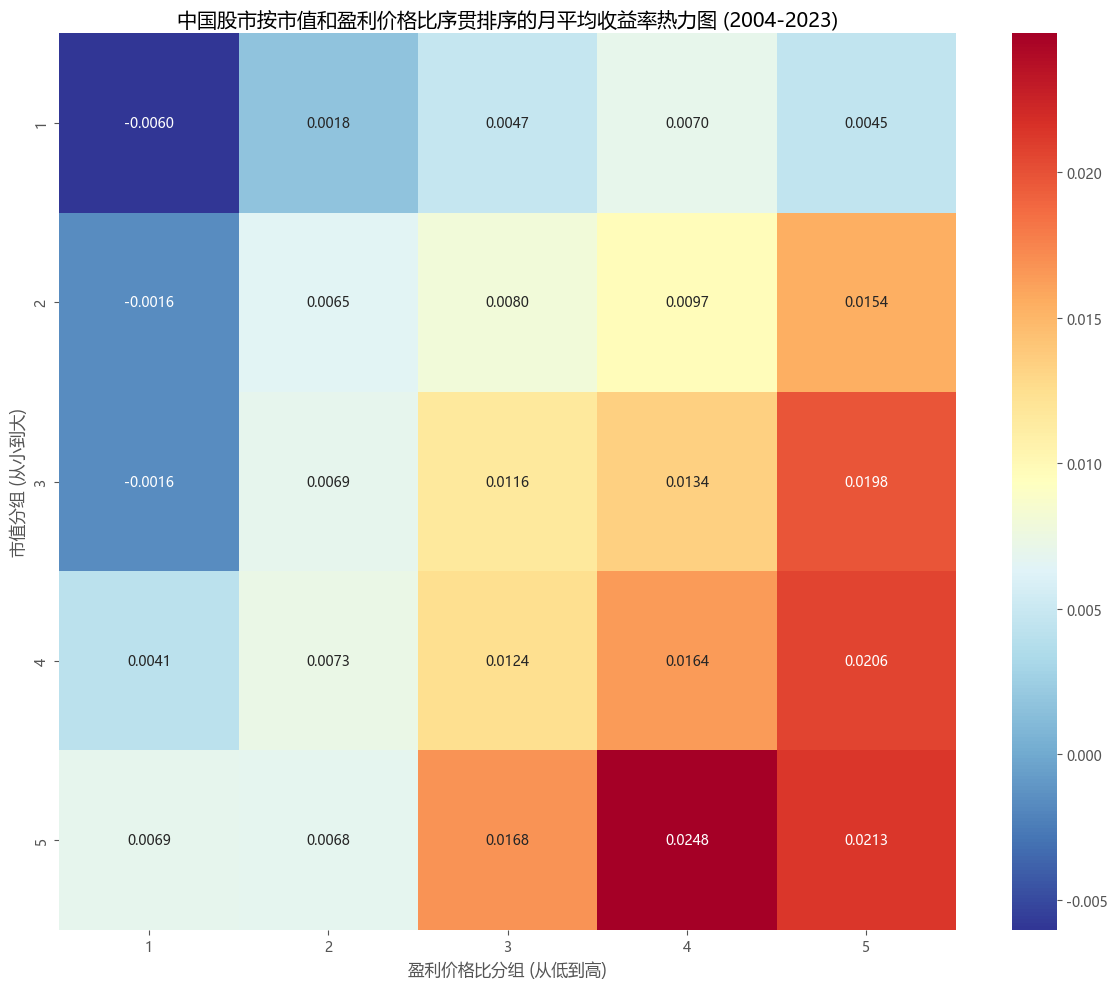
\includegraphics[width=0.8\textwidth]{./img/市值分组平均收益率.png}
\caption{不同市值和盈利价格比分组的月平均收益率热力图(2004-2023年)}
\label{fig:sequential_heatmap}
\end{figure}

图\ref{fig:sequential_heatmap}直观展示了不同市值和盈利价格比组合的月平均收益率分布,热力图清晰呈现了收益率随市值增加和盈利价格比降低而提高的趋势。从颜色变化可以明显观察到,右上角(大市值-低盈利价格比)区域的收益率明显高于左下角(小市值-高盈利价格比)区域,这一模式在整个样本期间保持一致,表明反向规模效应和反向价值效应是中国股市的稳健特征。

从价值维度考察,投资组合的平均月收益率随盈利价格比降低而增加,即从价值型向成长型转变时收益率呈上升趋势。最低盈利价格比组合(成长型)的月均收益率为1.63\%,显著高于最高盈利价格比组合(价值型)的0.04\%,两者差异达1.60\%(年化约19.20\%)。这表明中国股市存在系统性的反向价值效应,即成长型股票的表现优于价值型股票,同样与经典金融理论预期相反。

进一步分析投资组合间的交互效应,发现市值和盈利价格比因素之间存在复杂互动。以大市值-高盈利价格比(大盘价值)组合与小市值-低盈利价格比(小盘成长)组合为例,前者的月均收益率为0.69\%,显著高于后者的0.45\%,这进一步印证了在中国市场环境下大盘股的系统性优势。

最引人注目的是,大市值-次低盈利价格比组合(第5市值组-第4盈利价格比组)获得了所有25个组合中最高的月均收益率2.48\%,该现象表明市场对兼具一定成长性且规模较大的股票给予了特别青睐。这可能反映了机构投资者在中国市场中占据主导地位,而这些投资者倾向于配置流动性较好的大市值成长股。

综合来看,序贯排序分析的结果挑战了传统金融理论中的规模效应和价值效应假设,揭示了中国股市独特的定价机制,为投资策略设计与资产定价模型完善提供了重要实证依据。

\subsection{Fama-MacBeth横截面回归分析}

为深入检验市值、盈利价格比和CAPM Beta对股票收益率的解释能力,本研究采用Fama-MacBeth两阶段回归方法,分析了2004至2023年期间的中国A股横截面数据。表\ref{tab:fama_macbeth}报告了全样本期间及两个子样本期间的回归结果。

\begin{table}[htbp]
\centering
\caption{Fama-MacBeth回归结果}
\label{tab:fama_macbeth}
\begin{tabular}{lccc}
\toprule
 & 全样本期间 & 子期间1 & 子期间2 \\
 & (2004-2023) & (2004-2013) & (2014-2023) \\
\midrule
常数项 & -0.2014*** & -0.1834*** & -0.2315*** \\
 & (-6.33) & (-4.50) & (-4.53) \\
Beta & 0.0165** & 0.0175* & 0.0149 \\
 & (2.11) & (1.72) & (1.22) \\
对数流通市值 & 0.0096*** & 0.0090*** & 0.0106*** \\
 & (6.87) & (4.93) & (4.89) \\
盈利价格比 & -0.3733*** & -0.3717*** & -0.3760*** \\
 & (-7.14) & (-5.31) & (-4.89) \\
\midrule
平均$R^2$ & 0.0676 & 0.0761 & 0.0533 \\
观测月份数 & 192 & 120 & 72 \\
\bottomrule
\multicolumn{4}{l}{\scriptsize 注:括号内为t统计量;***、**、*分别表示在1\%、5\%和10\%的水平上显著。}
\end{tabular}
\end{table}

Fama-MacBeth回归结果强化并扩展了前述序贯排序分析的发现。在全样本期间(2004-2023年),三个关键因素均呈现出统计显著的系数。Beta系数为0.0165(t=2.11),表明系统性风险在中国股市定价中发挥着积极作用,符合CAPM理论预期的风险溢价存在。对数流通市值系数为显著正值0.0096(t=6.87),进一步证实了中国股市存在反向规模效应,即市值较大的股票在控制其他因素后仍能获得更高的预期收益。盈利价格比系数为显著负值-0.3733(t=-7.14),同样印证了市场存在反向价值效应,投资者更加青睐低盈利价格比(高市盈率)的成长型股票。

将全样本划分为两个子期间后,大多数结论保持稳健。对数流通市值和盈利价格比的系数在两个子期间均保持高度显著,且符号与全样本一致,表明这两种效应在中国股市中具有持续性。值得注意的是,Beta系数的显著性随时间有所减弱,从第一子期间的边际显著(t=1.72)降至第二子期间的不显著(t=1.22),这可能反映了系统性风险在近期对股票定价的影响有所减弱。

\begin{figure}[htbp]
\centering
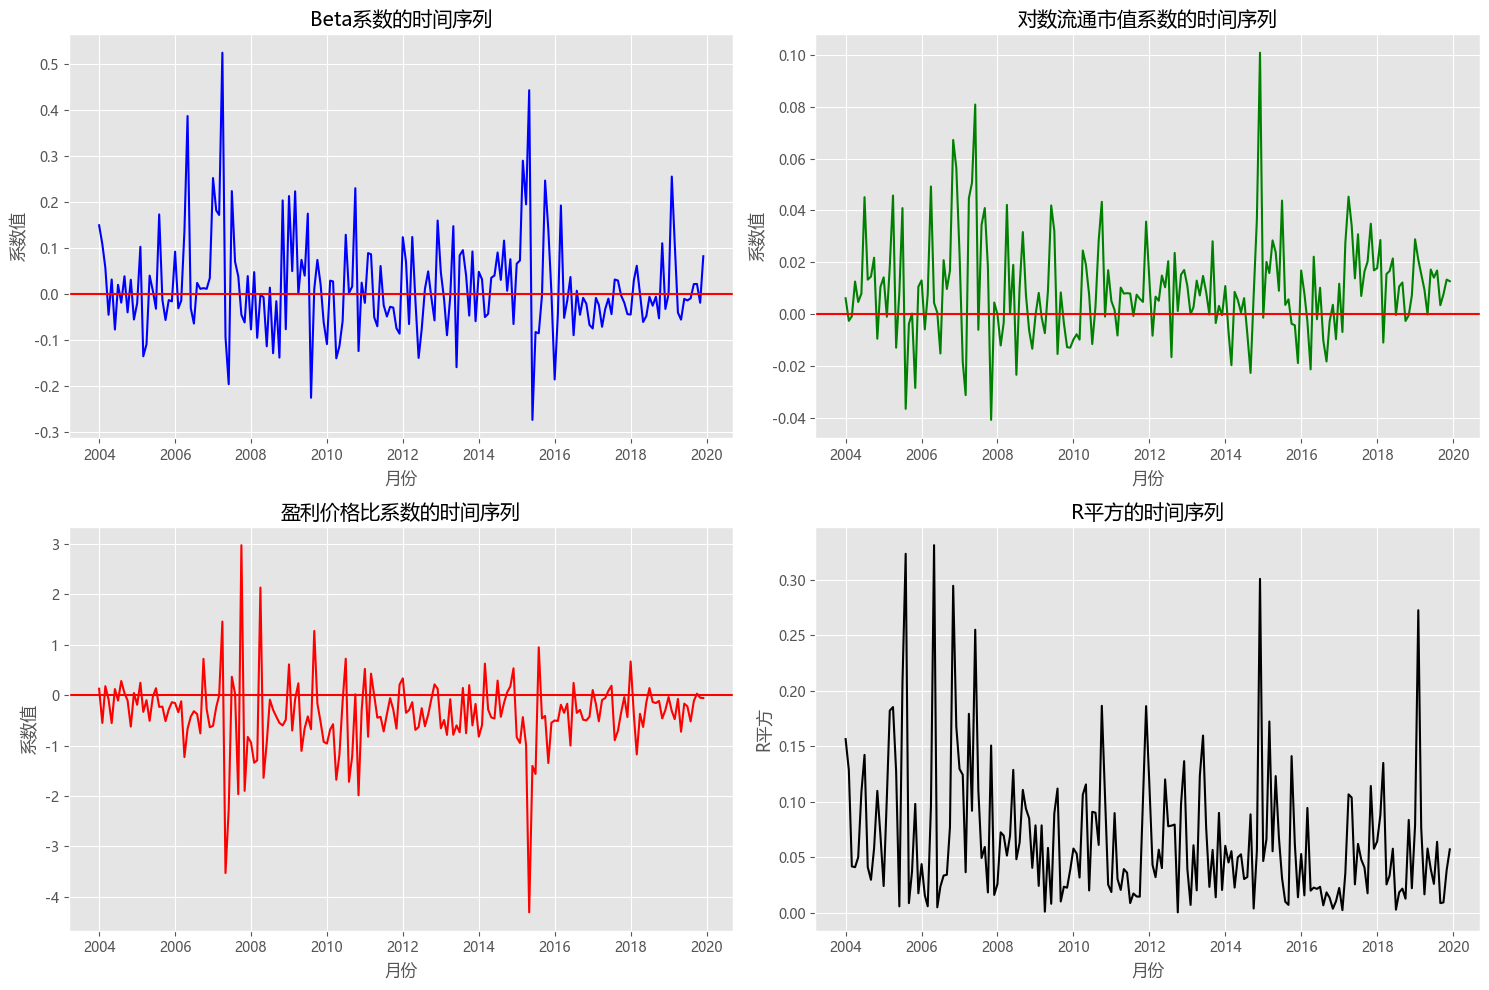
\includegraphics[width=0.8\textwidth]{./img/Beta系数的时间序列.png}
\caption{月度Fama-MacBeth回归系数的时间序列变化}
\label{fig:beta_timeseries}
\end{figure}

图\ref{fig:beta_timeseries}展示了回归系数随时间的波动模式,包括Beta系数、对数流通市值系数和盈利价格比系数的月度变化。尽管三个系数的整体平均值分别为正、正和负,但它们的时间序列均表现出较大波动性,这说明风险因子溢价在不同市场环境下存在显著变化。特别是在2008年金融危机和2015年股灾等市场剧烈波动期间,系数波动尤为明显,表明在极端市场环境下,各因子对股票收益率的影响会发生显著变化。图中右下角还展示了R平方的时间序列变化,反映了模型解释力在不同月份间的差异。

\begin{figure}[htbp]
\centering
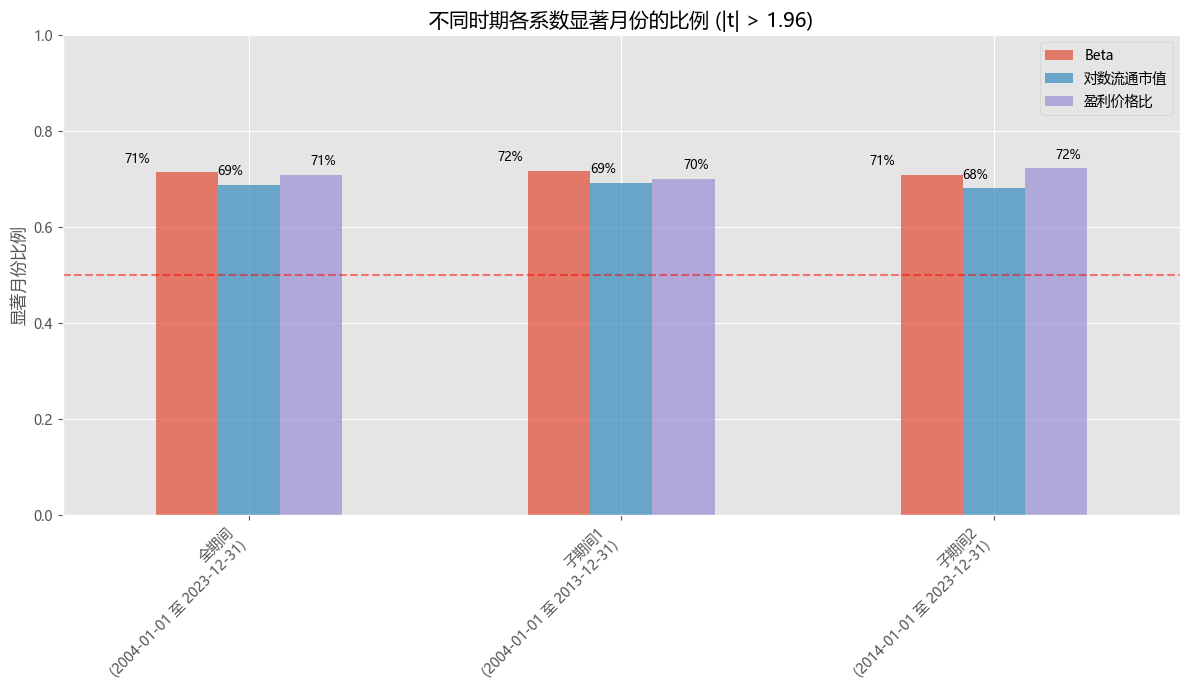
\includegraphics[width=0.8\textwidth]{./img/不同时期各系数显著月份的比例.png}
\caption{不同时期各系数显著月份的比例 (|t| > 1.96)}
\label{fig:coef_significance}
\end{figure}

图\ref{fig:coef_significance}展示了各风险因子在不同时期内显著月份的比例。在整个研究期间,Beta、对数流通市值和盈利价格比的显著月份比例分别为71\%、69\%和71\%,表明这些因素在大多数月份中对股票收益率具有显著解释力。同时,我们注意到第一子期间(2004-2013年)各因子的显著性与全样本期间基本一致,而第二子期间(2014-2023年)Beta因子和对数流通市值因子的显著性略有下降,这可能反映了近期市场定价机制的变化。

回归的平均R方为0.0676,表明模型整体解释了约6.76\%的横截面收益率变异。尽管数值相对较低,但与资产定价实证研究中通常观察到的横截面R方相当,反映了股票收益的高度随机性与预测难度。值得注意的是,第一子期间(2004-2013年)的平均R方(0.0761)显著高于第二子期间(2014-2023年)的0.0533,这可能表明近期市场效率的提高或其他未被模型捕捉的因素在近期发挥了更大作用。

总体而言,Fama-MacBeth回归结果与序贯排序分析高度一致,共同表明中国股市存在显著的反向规模效应和反向价值效应,同时CAPM预测的系统性风险溢价也得到了一定程度的支持。这些发现对理解中国股市的定价机制、构建适合中国市场的资产定价模型以及制定有效的投资策略均具有重要启示。

中国股市呈现反向规模效应和反向价值效应的原因可能多方面的。从制度环境看,中国股市的IPO审核制度对小市值公司形成一定壁垒,上市公司普遍规模较大,弱化了小市值溢价;从投资者结构看,机构投资者占比逐年提高,其偏好流动性较好的大市值股票的倾向助推了大市值股票的表现;从行为金融角度看,中国投资者可能对成长性预期存在系统性乐观偏差,推高了高市盈率股票的估值水平和实现收益率。

\section{讨论与结论}

本研究通过对Fama-French三因子模型的多维度检验、序贯排序分析以及Fama-MacBeth回归分析,系统考察了中国A股市场在2004至2023年间的资产定价特征与风险因子结构。研究发现揭示了中国股市资产定价机制的独特性及其与经典金融理论预期的显著差异。

首先,基于行业指数的FF三因子模型检验表明,该模型在时间序列维度展示出良好的解释力。无论是单资产检验还是GRS联合检验,均未能拒绝"截距项为零"的假设,表明市场、规模和价值三个系统性风险因素已能充分解释中国行业指数的超额收益。行业间差异分析揭示了风险暴露的行业异质性:银行业呈现低市场风险、负规模敏感性和正价值敏感性,而电气设备、化工等行业则表现出高市场风险、正规模敏感性和负价值敏感性,形成了价值型与成长型行业的鲜明对比。行业层面的发现支持了三因子模型在解释中国市场行业收益差异方面的有效性。

然而,当考察个股层面的定价机制时,本研究发现了与经典理论预期相反的市场特征。序贯排序分析揭示了中国股市存在显著的反向规模效应和反向价值效应。大市值股票的平均月收益率系统性高于小市值股票,两者差异高达1.29\%(年化约15.48\%);同时,低盈利价格比(高市盈率)的成长型股票表现显著优于高盈利价格比(低市盈率)的价值型股票,月度差异达1.60\%(年化约19.20\%)。最引人注目的是,大市值-次低盈利价格比组合获得了所有25个投资组合中最高的月均收益率(2.48\%),表明市场特别青睐兼具一定成长性且规模较大的股票。

Fama-MacBeth回归进一步证实了上述发现。在控制其他因素后,对数流通市值系数显著为正(0.0096,t=6.87),盈利价格比系数显著为负(-0.3733,t=-7.14),二者在不同子期间均保持稳健。同时,Beta系数整体上显著为正(0.0165,t=2.11),支持了CAPM预期的系统性风险溢价存在,但其显著性在近期有所减弱。各因子在研究期间内约70\%的月份中显著影响股票收益,表明这些因素在解释横截面收益差异方面具有持久性。

中国股市呈现反向规模效应和反向价值效应的原因可能是多方面的。从制度环境看,中国股市的IPO审核制度对小市值公司形成一定壁垒,上市公司普遍规模较大,弱化了小市值溢价;从投资者结构看,机构投资者占比逐年提高,其偏好流动性较好的大市值股票的倾向助推了大市值股票的表现;从行为金融角度看,中国投资者可能对成长性预期存在系统性乐观偏差,推高了高市盈率股票的估值水平和实现收益率。此外,监管政策与交易制度的特殊性也可能影响因子溢价的形成机制。

研究结果对资产定价理论与投资实践均有重要启示。在理论层面,传统基于美国市场构建的多因子模型可能不足以准确描述中国股市的风险-收益关系,需要发展更适合中国国情的本土化资产定价模型;在实践层面,投资者在中国市场进行投资时不应机械套用小市值和价值投资策略,而应考虑配置大市值成长型股票,尤其是那些兼具规模优势和成长潜力的股票。

本研究也存在一些局限性。首先,样本期间跨度较长,市场环境和监管政策在此期间发生了显著变化,可能影响结果的稳健性;其次,我们仅考虑了市值、盈利价格比和Beta三个主要因素,未能纳入动量、流动性、波动率等其他可能影响股票收益的因素;此外,本研究的样本选择可能存在幸存者偏差,因为只有在整个样本期间持续存在的股票才被纳入分析。

未来研究可在以下方向进一步深化:一是拓展模型框架,引入更多风险因子构建更全面的多因子模型;二是细分样本期间,分析不同市场状态下因子溢价的动态变化;三是探索因子溢价形成的微观机制,结合投资者行为、市场微观结构等视角深入解析中国股市的定价特征;四是研究资产定价异象的经济意义,分析反向规模效应和反向价值效应与中国宏观经济结构及政策环境的关联。通过这些努力,有望构建更加完善的中国股市资产定价理论体系,为投资者提供更为有效的决策依据。

\printbibliography[title=参考文献]

\section{附录}

本研究的核心代码如下:

\begin{lstlisting}[basicstyle=\small\ttfamily, breaklines=true, columns=fullflexible]
# ===== FF三因子模型的单资产时间序列检验 =====

# 估计三因子模型参数并检验是否满足FF三因子模型
def test_ff_model(industry_returns, factors):
    all_results = {}
    test_conclusions = {}
    
    for industry_name, returns in industry_returns.items():
        # 确保数据对齐
        aligned_data = pd.concat([returns, factors], axis=1, join='inner').dropna()
        
        # 计算超额收益率
        excess_returns = aligned_data.iloc[:, 0] - aligned_data['RF']
        
        # 准备自变量
        X = aligned_data[['MKT', 'SMB', 'HML']]
        X = sm.add_constant(X)
        
        # 运行OLS回归
        model = sm.OLS(excess_returns, X)
        results = model.fit()
        
        # 计算t统计量
        t_stats = calculate_t_statistic(results)
        
        # 模型检验:判断是否满足FF三因子模型
        alpha = results.params['const']
        alpha_pvalue = results.pvalues['const']
        r_squared = results.rsquared
        f_stat = results.fvalue
        f_pvalue = results.f_pvalue
        
        # 判断是否满足三因子模型
        alpha_significant = alpha_pvalue < 0.05
        model_significant = f_pvalue < 0.05
        
        if not alpha_significant and model_significant:
            conclusion = "满足FF三因子模型,a不显著,模型整体显著"
        elif alpha_significant and model_significant:
            conclusion = "不完全满足FF三因子模型,a显著,模型整体显著"
        elif not alpha_significant and not model_significant:
            conclusion = "不满足FF三因子模型,a不显著,但模型整体不显著"
        else:
            conclusion = "不满足FF三因子模型,a显著,模型整体不显著"
        
        # 存储结果
        all_results[industry_name] = t_stats
        test_conclusions[industry_name] = {
            'alpha': alpha, 'alpha_pvalue': alpha_pvalue, 
            'r_squared': r_squared, 'conclusion': conclusion,
            # 其他统计信息...
        }
    
    return all_results, test_conclusions


# ===== FF三因子模型的多资产联合检验 =====

# 使用GRS检验进行多资产联合检验
def multi_asset_ff_test(industry_returns, factors):
    # 1. 对每个行业单独进行OLS估计
    all_results = {}
    all_params = {}
    all_residuals = {}
    
    for industry, returns in industry_returns.items():
        # 对齐数据并进行回归
        aligned_data = pd.concat([returns, factors], axis=1, join='inner').dropna()
        excess_returns = aligned_data.iloc[:, 0] - aligned_data['RF']
        X = sm.add_constant(aligned_data[['MKT', 'SMB', 'HML']])
        model = sm.OLS(excess_returns, X)
        results = model.fit()
        
        # 存储结果
        all_results[industry] = results
        all_params[industry] = results.params
        all_residuals[industry] = results.resid
    
    # 2. 计算GRS统计量
    # 提取所有行业的alpha值
    alphas = np.array([params['const'] for params in all_params.values()])
    
    # 计算残差的协方差矩阵
    T = len(next(iter(all_residuals.values())))  # 样本数
    residuals_df = pd.DataFrame(all_residuals)
    Sigma = residuals_df.cov()  # 残差协方差矩阵
    
    # 计算GRS检验公式相关参数
    N = len(all_results)  # 资产数量
    K = 3  # 三个因子
    mu_k = np.array([factors['MKT'].mean(), factors['SMB'].mean(), factors['HML'].mean()])
    factor_data = factors[['MKT', 'SMB', 'HML']]
    Omega = factor_data.cov()
    
    # 计算GRS统计量
    Omega_inv = np.linalg.inv(Omega)
    mu_Omega_inv_mu = np.dot(np.dot(mu_k, Omega_inv), mu_k)
    Sigma_inv = np.linalg.inv(Sigma)
    alpha_Sigma_inv_alpha = np.dot(np.dot(alphas, Sigma_inv), alphas)
    GRS_stat = ((T - N - K) / N) * (1 + mu_Omega_inv_mu)**(-1) * alpha_Sigma_inv_alpha
    
    # 计算p值 (F分布,自由度为N和T-N-K)
    p_value = 1 - stats.f.cdf(GRS_stat, N, T - N - K)
    
    joint_test_result = {
        'GRS_stat': GRS_stat, 'p_value': p_value,
        'reject_H0': p_value < 0.05, 'N': N, 'T': T, 'K': K,
        # 其他统计信息...
    }
    
    # 3. 整理单个资产检验结果
    individual_results = {}
    for industry, results in all_results.items():
        individual_results[industry] = {
            'alpha': results.params['const'],
            'alpha_tstat': results.tvalues['const'],
            'beta_mkt': results.params['MKT'],
            'beta_smb': results.params['SMB'],
            'beta_hml': results.params['HML'],
            'r_squared': results.rsquared,
            # 其他统计信息...
        }
    
    return joint_test_result, individual_results


# ===== 市值与盈利价格比的序贯排序分析 =====

# 序贯排序函数:先按市值排序,再按盈利价格比排序
def sequential_sort(df, date_col='日期_Date', return_col='月收益率_Monret', 
                   first_sort_col='流通市值', second_sort_col='盈利价格比', n_groups=5):
    results = []
    all_months = sorted(df[date_col].unique())
    
    for date in all_months:
        # 获取当月的数据
        month_data = df[df[date_col] == date].copy()
        
        # 确保数据足够
        if len(month_data) < n_groups * 2:
            continue
            
        # 删除无效值和异常值
        month_data = month_data.dropna(subset=[first_sort_col, second_sort_col, return_col])
        month_data = month_data[(month_data[return_col] > -0.5) & (month_data[return_col] < 0.5)]
        month_data = month_data[month_data[second_sort_col] > 0]
        
        if len(month_data) < n_groups * 2:
            continue
        
        try:
            # 先按流通市值排序分组(从小到大)
            month_data['size_rank'] = pd.qcut(month_data[first_sort_col], n_groups, labels=False, duplicates='drop')
            
            # 在每个流通市值分组内,按盈利价格比排序再分组(从高到低)
            for size_rank, size_group in month_data.groupby('size_rank'):
                if len(size_group) < n_groups:
                    continue
                
                # 负号使盈利价格比从高到低排序
                size_group['ep_rank'] = pd.qcut(-size_group[second_sort_col], n_groups, labels=False, duplicates='drop')
                
                # 计算每个分组的平均收益率
                for ep_rank, ep_group in size_group.groupby('ep_rank'):
                    avg_return = ep_group[return_col].mean()
                    results.append({
                        '日期': date,
                        '市值分组': size_rank + 1,  # 从1开始
                        '盈利价格比分组': ep_rank + 1,  # 从1开始
                        '平均收益率': avg_return,
                        '股票数量': len(ep_group)
                    })
        except Exception as e:
            continue
    
    results_df = pd.DataFrame(results)
    return results_df

# 计算最终的各分组时间序列平均收益率
def calculate_final_results(sorted_results):
    # 按市值和盈利价格比分组计算平均收益率
    final_results = sorted_results.groupby(['市值分组', '盈利价格比分组'])['平均收益率'].mean().reset_index()
    
    # 转换为宽格式表格
    pivot_table = final_results.pivot(index='市值分组', columns='盈利价格比分组', values='平均收益率')
    
    # 确保所有的分组都存在,填充缺失值
    all_size_groups = range(1, 6)  # 1到5
    all_ep_groups = range(1, 6)    # 1到5
    pivot_table = pivot_table.reindex(index=all_size_groups, columns=all_ep_groups)
    
    # 添加边缘平均值
    size_means = sorted_results.groupby('市值分组')['平均收益率'].mean()
    ep_means = sorted_results.groupby('盈利价格比分组')['平均收益率'].mean()
    overall_mean = sorted_results['平均收益率'].mean()
    
    pivot_table['市值组平均'] = size_means
    
    # 计算列平均值并添加到表格底部
    ep_means_row = pd.Series(index=pivot_table.columns)
    for col in all_ep_groups:
        if col in pivot_table.columns:
            ep_means_row[col] = pivot_table[col].mean()
    ep_means_row['市值组平均'] = overall_mean
    
    pivot_table.loc['盈利价格比组平均'] = ep_means_row
    
    return pivot_table


# ===== Fama-MacBeth横截面回归分析 =====

# 计算股票Beta值
def calculate_beta(df, window=36):
    # 计算每个月的市场平均收益率(等权)
    market_returns = df.groupby('日期_Date')['月收益率_Monret'].mean().reset_index()
    market_returns.columns = ['日期_Date', '市场收益率']
    
    # 合并市场收益率到主数据框
    df_merged = pd.merge(df, market_returns, on='日期_Date', how='left')
    
    # 计算超额收益率
    df_merged['超额收益率'] = df_merged['月收益率_Monret'] - df_merged['月无风险收益率_Monrfret']
    df_merged['市场超额收益率'] = df_merged['市场收益率'] - df_merged['月无风险收益率_Monrfret']
    
    # 为每只股票计算Beta值
    beta_results = []
    
    for stock in df_merged['股票代码_Stkcd'].unique():
        stock_data = df_merged[df_merged['股票代码_Stkcd'] == stock].copy()
        stock_data = stock_data.sort_values('日期_Date')
        
        # 使用滚动窗口计算Beta
        for j in range(window, len(stock_data) + 1):
            window_data = stock_data.iloc[j-window:j]
            current_date = window_data.iloc[-1]['日期_Date']
            
            try:
                # 执行回归计算Beta
                X = sm.add_constant(window_data['市场超额收益率'])
                y = window_data['超额收益率']
                model = sm.OLS(y, X).fit()
                beta = model.params['市场超额收益率']
                
                # 限制Beta值在合理范围
                if beta < -3 or beta > 3:
                    beta = 1.0
            except:
                beta = 1.0
            
            beta_results.append({
                '股票代码_Stkcd': stock,
                '日期_Date': current_date,
                'Beta': beta
            })
    
    # 将结果转换为DataFrame并合并到原始数据
    beta_df = pd.DataFrame(beta_results)
    df_with_beta = pd.merge(df, beta_df, on=['股票代码_Stkcd', '日期_Date'], how='left')
    
    # 填充缺失的Beta值
    df_with_beta['Beta'] = df_with_beta['Beta'].fillna(1.0)
    
    return df_with_beta

# Fama-MacBeth两阶段回归
def fama_macbeth_regression(df, start_date, end_date):
    # 筛选时间范围内的数据
    df = df[(df['日期_Date'] >= start_date) & (df['日期_Date'] <= end_date)].copy()
    
    # 对所有变量进行缩尾处理(处理极端值)
    for col in ['对数流通市值', '盈利价格比', 'Beta']:
        df[col + '_winsorized'] = df.groupby('年月')[col].transform(
            lambda x: x.clip(lower=x.quantile(0.01), upper=x.quantile(0.99))
        )
    
    # 获取所有唯一的月份
    all_months = df['日期_Date'].dt.to_period('M').unique()
    all_months = sorted(all_months)
    
    # 用于存储每个月的横截面回归结果
    monthly_results = []
    
    # 对每个月执行横截面回归
    for month in all_months:
        month_str = str(month)
        month_start = month_str + '-01'
        month_end = pd.Period(month).asfreq('D', 'end').strftime('%Y-%m-%d')
        
        # 获取当月数据
        month_data = df[(df['日期_Date'] >= month_start) & (df['日期_Date'] <= month_end)].copy()
        
        # 确保数据充足并删除缺失值
        if len(month_data) < 30:
            continue
        
        month_data = month_data.dropna(subset=['月收益率_Monret', '对数流通市值_winsorized', 
                                               '盈利价格比_winsorized', 'Beta_winsorized'])
        
        if len(month_data) < 30:
            continue
        
        try:
            # 准备回归数据
            X = sm.add_constant(month_data[['Beta_winsorized', '对数流通市值_winsorized', '盈利价格比_winsorized']])
            y = month_data['月收益率_Monret']
            
            # 执行OLS回归
            model = sm.OLS(y, X)
            results = model.fit()
            
            # 收集结果
            monthly_results.append({
                '月份': month_str,
                '常数项': results.params['const'],
                'Beta': results.params['Beta_winsorized'],
                '对数流通市值': results.params['对数流通市值_winsorized'],
                '盈利价格比': results.params['盈利价格比_winsorized'],
                '常数项_t值': results.tvalues['const'],
                'Beta_t值': results.tvalues['Beta_winsorized'],
                '对数流通市值_t值': results.tvalues['对数流通市值_winsorized'],
                '盈利价格比_t值': results.tvalues['盈利价格比_winsorized'],
                'R平方': results.rsquared,
                '样本数': len(month_data)
            })
        except Exception as e:
            continue
    
    # 将结果转换为DataFrame
    fm_results = pd.DataFrame(monthly_results)
    
    # 计算Fama-MacBeth第二阶段结果(时间序列平均值和t统计量)
    coef_means = fm_results[['常数项', 'Beta', '对数流通市值', '盈利价格比']].mean()
    coef_stds = fm_results[['常数项', 'Beta', '对数流通市值', '盈利价格比']].std()
    n_periods = len(fm_results)
    coef_t_stats = coef_means / (coef_stds / np.sqrt(n_periods))
    
    # 输出结果
    print("\nFama-MacBeth回归结果(时间序列平均值):")
    for coef, mean_val, t_stat in zip(['常数项', 'Beta', '对数流通市值', '盈利价格比'], 
                                      coef_means, coef_t_stats):
        print(f"{coef}: {mean_val:.6f} (t = {t_stat:.2f})")
    
    print(f"平均R平方: {fm_results['R平方'].mean():.4f}")
    
    return fm_results

# 按日期区间运行Fama-MacBeth回归并比较不同时期的结果
def run_fama_macbeth_with_subperiods(df, full_period, subperiods):
    # 分割时间区间
    full_start, full_end = full_period.split(':')
    
    # 完整期间回归
    full_results = fama_macbeth_regression(df, start_date=full_start, end_date=full_end)
    
    # 子期间回归
    subperiod_results = []
    for period in subperiods:
        start_date, end_date = period.split(':')
        sub_results = fama_macbeth_regression(df, start_date=start_date, end_date=end_date)
        subperiod_results.append(sub_results)
    
    return full_results, subperiod_results
\end{lstlisting}

\end{document}